% Copyright (c) Patrick Hall (jphall@gwu.edu), 2026-27. CC BY-NC-SA 4.0.
\documentclass[aspectratio=169]{beamer}
\usetheme{Singapore}
\definecolor{brand}{RGB}{45,110,191}
\definecolor{hrgray}{RGB}{100,100,100}
\setbeamercolor{structure}{fg=brand}
\setbeamercolor{title}{fg=hrgray}
\setbeamercolor{subtitle}{fg=brand}
\setbeamercolor{frametitle}{fg=hrgray}
\setbeamercolor{block title}{fg=white,bg=brand}
\setbeamercolor{block body}{bg=black!2}
\usepackage[T1]{fontenc}
\usepackage[utf8]{inputenc}
\usepackage{lmodern,microtype,graphicx,booktabs,tikz,amsmath}
\usepackage[backend=biber,style=authoryear,maxcitenames=2,maxbibnames=10,doi=false,isbn=false]{biblatex}
\addbibresource{references.bib}
\DeclareBibliographyCategory{referencesone}
\DeclareBibliographyCategory{referencestwo}
\addtocategory{referencesone}{Holtzman2020CuriousCase,Mikolov2013EfficientEstimationWord,Ouyang2022TrainingLanguageModels,PromontoryAI2026Practicum,Rafailov2023DirectPreferenceOptimization}
\addtocategory{referencestwo}{Sennrich2016NeuralMachineTranslation,Snell2024ScalingLLMTestTime,Vaswani2017AttentionAllYou,Wei2022ChainThoughtPrompting}
\renewcommand*{\mkbibacro}[1]{#1}
\renewcommand*{\bibfont}{\scriptsize}
\usetikzlibrary{positioning,arrows.meta}
\setbeamertemplate{navigation symbols}{}
\setbeamertemplate{bibliography item}{}
\setbeamertemplate{frametitle continuation}{}
\setbeamertemplate{footline}{\leavevmode\hbox{\begin{beamercolorbox}[wd=.5\paperwidth,ht=3ex,dp=1ex,left]{author in head/foot}\hspace{0.8ex}
\includegraphics[height=.5cm]{../../asset/gw_logo.png}\end{beamercolorbox}\begin{beamercolorbox}[wd=.5\paperwidth,ht=3ex,dp=1ex,right]{date in head/foot}\insertframenumber/\inserttotalframenumber\hspace{2ex}\end{beamercolorbox}}}
\title{Lecture 1: LLM and transformer foundations}
\author[Patrick Hall]{\textbf{Patrick Hall}}
\institute{Department of Decision Sciences}
\date{\today}
\newcommand{\E}{\mathbf{E}}
\newcommand{\x}{\mathbf{x}}
\newcommand{\y}{\mathbf{y}}
\newcommand{\slidesource}[1]{\vfill\tiny\color{hrgray}Source: #1.}
\newcommand{\visualdescription}[1]{\par\vspace{.25em}{\centering\tiny\color{hrgray}#1\par}}
\begin{document}

\begin{frame}
  \titlepage
  \vspace{-.75em}
  \centering\scriptsize \textcopyright\ 2026--27 Patrick Hall (jphall@gwu.edu). Some rights reserved. Text and copy are licensed under a \href{https://creativecommons.org/licenses/by-nc-sa/4.0/}{Creative Commons Attribution-NonCommercial-ShareAlike 4.0 International License (CC BY-NC-SA 4.0)}.
  \begin{tikzpicture}[remember picture,overlay]
    \node[opacity=.08] at (current page.center) {
\includegraphics[width=.55\paperwidth]{../../asset/gw_logo.png}};
  \end{tikzpicture}
\end{frame}

\begin{frame}{Agenda}
  \tableofcontents
\end{frame}

\section{Predicting the next word}

\begin{frame}{Tokenization turns text into supervised data}
\small
\begin{columns}[T]
\column{.53\textwidth}
\textbf{Vocabulary} $\mathcal V=\{\texttt{<pad>},\texttt{see},\texttt{spot},\texttt{run},\texttt{fast},\texttt{<eot>}\}$, with IDs $0,\ldots,5$.
\vspace{.5em}

The sentence \texttt{see spot run fast <eot>} becomes $[1,2,3,4,5]$. \textbf{Context-window length: $L=4$ tokens.} Each prediction uses at most the four most recent token IDs; left-pad shorter prefixes with $0$:
\vspace{.4em}
\begin{center}\tiny\setlength{\tabcolsep}{2pt}
\begin{tabular}{c|c|c}
prefix & $\x^{(i)}\in\mathcal X\subset\{0,\ldots,5\}^{4}$ & $y^{(i)}\in\mathcal Y=\mathcal V$\\ \midrule
\texttt{see} & $[0,0,0,1]$ & \texttt{spot} (2)\\
\texttt{see spot} & $[0,0,1,2]$ & \texttt{run} (3)\\
\texttt{see spot run} & $[0,1,2,3]$ & \texttt{fast} (4)\\
\texttt{see spot run fast} & $[1,2,3,4]$ & \texttt{<eot>} (5)
\end{tabular}
\end{center}
\column{.43\textwidth}
\begin{block}{Supervised learning}
The observed dataset is $\mathbf X,\mathbf Y=\{(\x^{(i)},y^{(i)})\}_{i=0}^{N-1}$. Training produces a model $g$ whose predictions $g(\mathbf X)=\hat{\mathbf Y}$ approximate $\mathbf Y$.
\end{block}
\end{columns}
\end{frame}

\begin{frame}{A one-hidden-layer MLP scores every possible next token}
\small
\begin{columns}[T]
\column{.58\textwidth}
\scriptsize
Each ID indexes a learned row of an embedding table $\E\in\mathbb R^{6\times2}$.\\[.35em]
For $\x=[x_1,\ldots,x_4]$:
\[
\E_{\x}=[\E_{x_1};\E_{x_2};\E_{x_3};\E_{x_4}]\in\mathbb R^{4\times2},
\quad \mathbf z=\operatorname{vec}(\E_{\x})\in\mathbb R^8.
\]
\[
\mathbf h=\tanh(\mathbf W_1\mathbf z+\mathbf b_1),
\quad \mathbf s=\mathbf W_2\mathbf h+\mathbf b_2,
\quad \hat{\mathbf p}=\operatorname{softmax}(\mathbf s).
\]
Here $\hat p_j=P_g(Y=j\mid\x)$; categorical cross-entropy (multiclass log loss) for one example is $-\log \hat p_{y^{(i)}}$.\\[.35em]
Gradient descent updates $\E,\mathbf W_1,\mathbf b_1,\mathbf W_2,\mathbf b_2$.\\[.35em]
\textbf{Loss example:} if $y^{(i)}=4$ and $\hat p_4=0.80$, then $-\log(0.80)\approx0.223$.\\[1em]
\textbf{Layer flow:} $4$ token IDs $\rightarrow 4\times2=8$ embedding coordinates $\rightarrow 4$ \texttt{tanh} units $\rightarrow 6$ next-token probabilities.\\[.35em]
Each layer's output matches the next layer's input: $(4,2)\rightarrow8\rightarrow4\rightarrow6$.
\column{.38\textwidth}
\centering
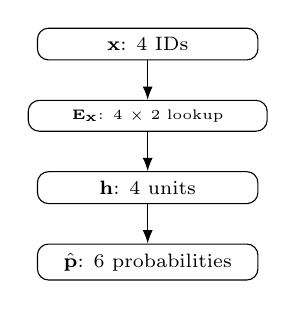
\begin{tikzpicture}[>=Latex, node distance=5mm, every node/.style={font=\scriptsize}]
\node[draw,rounded corners,align=center,minimum width=28mm] (x) {$\x$: 4 IDs};
\node[draw,rounded corners,align=center,minimum width=28mm,text width=28mm,font=\tiny,below=of x] (e) {$\E_{\x}$: $4\times2$ lookup};
\node[draw,rounded corners,align=center,minimum width=28mm,below=of e] (h) {$\mathbf h$: 4 units};
\node[draw,rounded corners,align=center,minimum width=28mm,below=of h] (p) {$\hat{\mathbf p}$: 6 probabilities};
\draw[->] (x)--(e); \draw[->] (e)--(h); \draw[->] (h)--(p);
\end{tikzpicture}
\vspace{1em}
\begin{block}{Why not predict ID 4 directly?}
IDs are labels, not ordered quantities. Six softmax probabilities define a categorical prediction.
\end{block}
\end{columns}
\end{frame}

\begin{frame}[t]{The example MLP}
\centering
\small
For $\x=[0,1,2,3]$ (\texttt{<pad>, see, spot, run}), the context-window length is $L=4$: each token contributes two learned coordinates. Every embedding coordinate connects to every hidden unit; every hidden unit scores every vocabulary item.
\vspace{.4em}

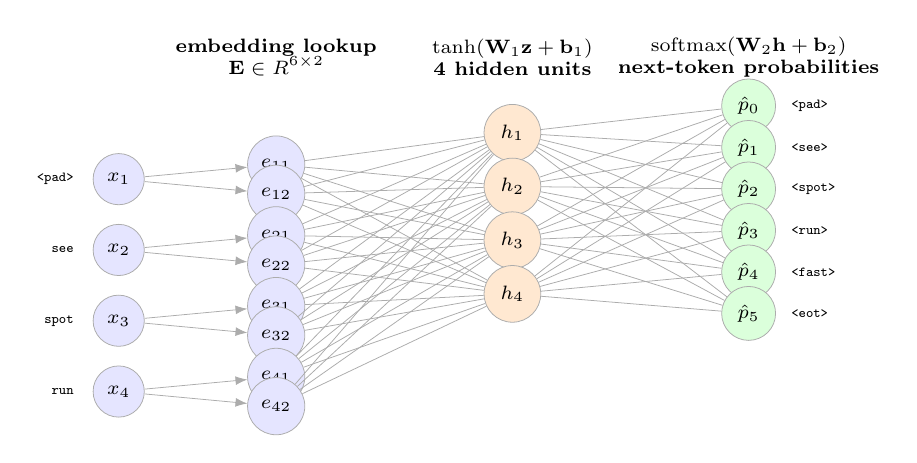
\begin{tikzpicture}[>=Latex, x=1cm, y=.62cm,
  input/.style={circle,draw,fill=blue!10,minimum size=6.2mm,font=\scriptsize},
  hidden/.style={circle,draw,fill=orange!18,minimum size=7.2mm,font=\scriptsize},
  output/.style={circle,draw,fill=green!14,minimum size=6.5mm,font=\scriptsize},
  every path/.style={draw=gray!65,line width=.28pt}]
% Token positions and their two-dimensional embeddings.
\foreach \pos/\token in {1/{<pad>},2/{see},3/{spot},4/{run}} {
  \node[input] (t\pos) at (0,{5.4-1.45*\pos}) {$x_\pos$};
  \node[font=\tiny,anchor=east] at (-.45,{5.4-1.45*\pos}) {\texttt{\token}};
  \node[input] (e\pos a) at (2,{5.7-1.45*\pos}) {$e_{\pos1}$};
  \node[input] (e\pos b) at (2,{5.1-1.45*\pos}) {$e_{\pos2}$};
  \draw[->] (t\pos) -- (e\pos a); \draw[->] (t\pos) -- (e\pos b);
}
% Four hidden units.
\foreach \n/\yy in {1/4.9,2/3.8,3/2.7,4/1.6} {
  \node[hidden] (h\n) at (5,\yy) {$h_\n$};
}
% Six categorical softmax outputs.
\foreach \n/\word/\yy in {0/{pad}/5.45,1/{see}/4.6,2/{spot}/3.75,3/{run}/2.9,4/{fast}/2.05,5/{eot}/1.2} {
  \node[output] (o\n) at (8,\yy) {$\hat p_\n$};
  \node[font=\tiny,anchor=west] at (8.42,\yy) {\texttt{<\word>}};
}
% Dense affine layers; the activations and softmax are named above their layers.
\foreach \pos in {1,2,3,4} {\foreach \coord in {a,b} {\foreach \n in {1,2,3,4} {\draw (e\pos\coord) -- (h\n);}}}
\foreach \n in {1,2,3,4} {\foreach \out in {0,1,2,3,4,5} {\draw (h\n) -- (o\out);}}
\node[align=center,font=\scriptsize\bfseries] at (2,6.45) {embedding lookup\\$\E\in\mathbb R^{6\times2}$};
\node[align=center,font=\scriptsize\bfseries] at (5,6.45) {$\tanh(\mathbf W_1\mathbf z+\mathbf b_1)$\\4 hidden units};
\node[align=center,font=\scriptsize\bfseries] at (8,6.45) {$\operatorname{softmax}(\mathbf W_2\mathbf h+\mathbf b_2)$\\next-token probabilities};
\end{tikzpicture}

\vspace{-.7em}
\scriptsize The output row with the largest probability is decoded; in this training example, $\arg\max_j\hat p_j=4$, or \texttt{fast}.
\end{frame}

\begin{frame}{Detokenization makes the prediction readable}
\small
For the context \texttt{see spot run}, tokenization gives $\x=[0,1,2,3]$. After the MLP:
\[
\hat{\mathbf p}=\left[\hat p_{\texttt{<pad>}},\hat p_{\texttt{see}},\hat p_{\texttt{spot}},\hat p_{\texttt{run}},\hat p_{\texttt{fast}},\hat p_{\texttt{<eot>}}\right].
\]
\begin{columns}[T]
\column{.55\textwidth}
\begin{block}{Decode}
$\hat y=\arg\max_{j\in\{0,\ldots,5\}}\hat p_j$ is an ID. The inverse vocabulary map converts it back to text: $\hat y=4\mapsto\texttt{fast}$.
\end{block}
\begin{block}{Generate another token}
Append the decoded ID, shift the context to $[1,2,3,4]$, and predict again. A learned model should then assign high probability to \texttt{<eot>}.
\end{block}
\column{.39\textwidth}\centering
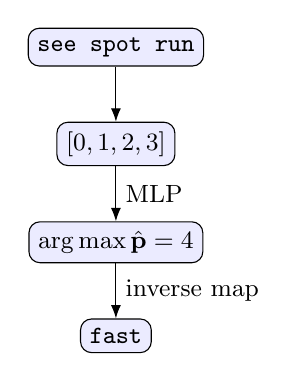
\begin{tikzpicture}[>=Latex, every node/.style={font=\small}]
\node[draw,rounded corners,fill=blue!8] (a) {\texttt{see spot run}};
\node[draw,rounded corners,fill=blue!8,below=7mm of a] (b) {$[0,1,2,3]$};
\node[draw,rounded corners,fill=blue!8,below=7mm of b] (c) {$\arg\max\hat{\mathbf p}=4$};
\node[draw,rounded corners,fill=blue!8,below=7mm of c] (d) {\texttt{fast}};
\draw[->] (a)--(b); \draw[->] (b)--node[right]{MLP}(c); \draw[->] (c)--node[right]{inverse map}(d);
\end{tikzpicture}
\end{columns}
\end{frame}

\begin{frame}{What the two-dimensional embedding plot shows}
\small
\begin{columns}[T]
\column{.56\textwidth}
The notebook plots the learned $2$-D vector $\E_j\in\mathbb R^2$ associated with each vocabulary token after training.
\begin{itemize}
\item Tokens used in similar predictive contexts can become nearby; this is an empirical pattern, not a guarantee in a tiny dataset.
\item The axes themselves have no fixed linguistic interpretation: rotating or reflecting all embeddings can leave equivalent downstream behavior after compensating weights.
\item The plot is useful for inspecting the representation, while softmax probabilities remain the model's next-word output.
\end{itemize}
\column{.39\textwidth}
\begin{block}{Notebook correspondence}
Same vocabulary, four padded examples, $2$-D token embeddings, $4$ hidden units, cross-entropy training, decoding, and an embedding scatter plot.
\end{block}
\vspace{1em}
\centering\Large text $\rightarrow$ IDs $\rightarrow$ embeddings $\rightarrow$ probabilities $\rightarrow$ text
\end{columns}
\end{frame}

\section{Transfomer Concepts}

\begin{frame}{Tokens are the model's units of text}
\small
\begin{columns}[T]
\column{.47\textwidth}
\begin{itemize}
  \item A tokenizer maps text to IDs from a fixed vocabulary; detokenization reverses the map.
  \item Subword vocabularies reuse frequent pieces, so rare words need not become unknown words.
  \item Context limits and API usage are measured in tokens, not words or characters.
\end{itemize}
\column{.49\textwidth}
\centering
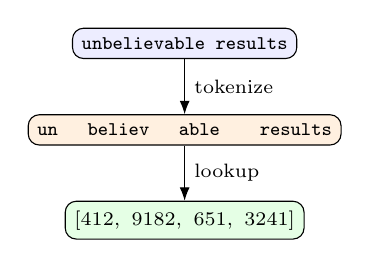
\begin{tikzpicture}[>=Latex,node distance=3mm,every node/.style={font=\scriptsize}]
  \node[draw,rounded corners,fill=blue!7] (text) {\texttt{unbelievable results}};
  \node[draw,rounded corners,fill=orange!12,below=7mm of text] (parts) {\texttt{un} \quad \texttt{believ} \quad \texttt{able} \quad \texttt{ results}};
  \node[draw,rounded corners,fill=green!10,below=7mm of parts] (ids) {$[412,\ 9182,\ 651,\ 3241]$};
  \draw[->] (text)--node[right]{tokenize}(parts);
  \draw[->] (parts)--node[right]{lookup}(ids);
\end{tikzpicture}
\vspace{1em}

\begin{block}{Important consequence}
The same visible word can use different token pieces across tokenizers; token counts therefore depend on the model's vocabulary.
\end{block}
\end{columns}
\slidesource{\textcite{Sennrich2016NeuralMachineTranslation}, \href{https://aclanthology.org/P16-1162/}{subword units}}
\end{frame}

\begin{frame}{Embeddings turn discrete IDs into learned vectors}
\small
\begin{columns}[c]
\column{.37\textwidth}
An embedding table maps token ID $j$ to a dense vector $\E_j\in\mathbb R^d$.
\begin{itemize}
  \item Vectors are learned from predictive objectives.
  \item Relative geometry can encode useful regularities.
  \item In a transformer, position information is added or otherwise incorporated before attention.
\end{itemize}
\column{.59\textwidth}
\centering
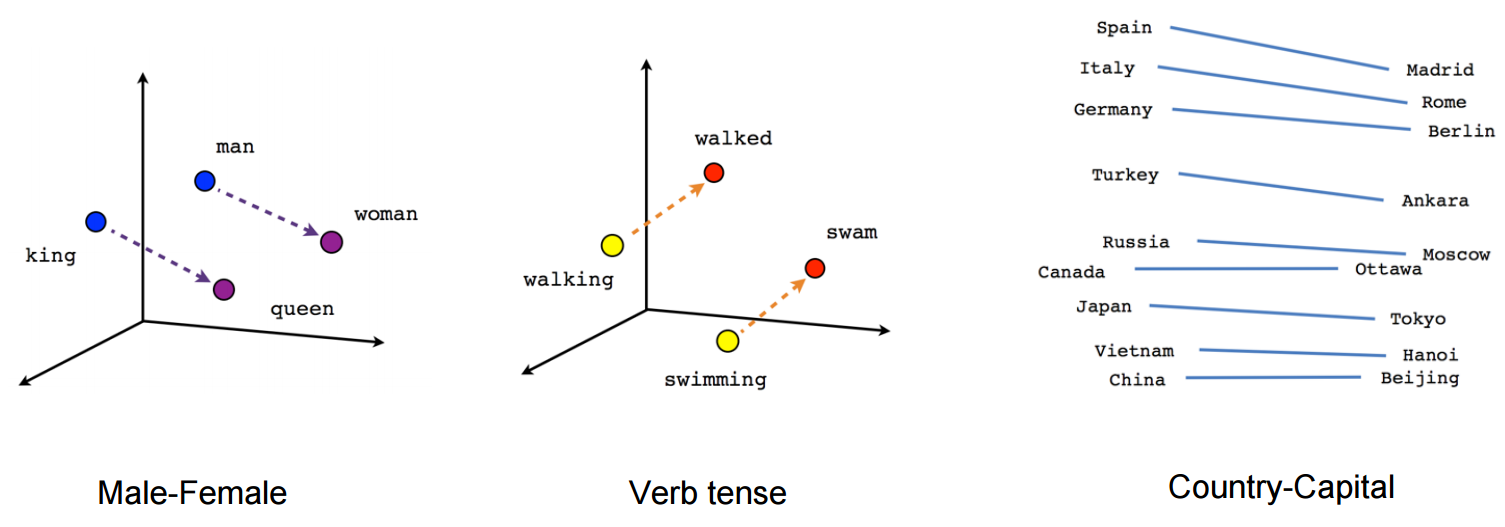
\includegraphics[width=\linewidth]{asset/word2vec_relations.png}
\visualdescription{Illustrative embedding relations: similar transformations appear as related vector offsets.}
\end{columns}
\slidesource{\textcite{Mikolov2013EfficientEstimationWord}, \href{https://arxiv.org/abs/1301.3781}{distributed word representations}}
\end{frame}

\begin{frame}{Attention mixes information across token positions}
\small
\begin{columns}[c]
\column{.37\textwidth}
\footnotesize
At each token position, learned linear transformations map the input representation to a query, key, and value vector:
{\scriptsize
\setlength{\abovedisplayskip}{.2em}
\setlength{\belowdisplayskip}{.1em}
\[
\operatorname{Attn}(Q,K,V)=
\operatorname{softmax}\!\left(\frac{QK^\top}{\sqrt{d_k}}\right)V.
\]
}
\begin{itemize}
  \setlength{\topsep}{.1em}
  \setlength{\itemsep}{.05em}
  \item For each query, softmax weights determine how value vectors are mixed into the output.
  \item Multiple heads can learn different relationships.
  \item In self-attention, queries, keys, and values are derived from the same sequence of tokens.
\end{itemize}
\column{.59\textwidth}
\centering
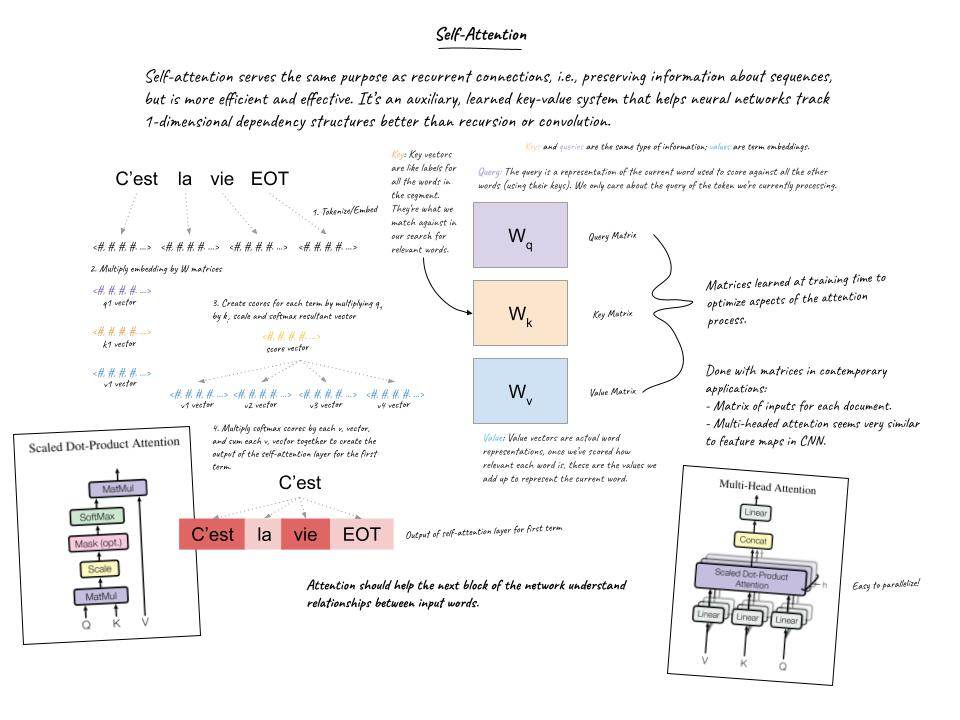
\includegraphics[width=.87\linewidth]{asset/self_attention.jpg}
\visualdescription{Queries score keys; attention weights mix value vectors across token positions.}
\end{columns}
\slidesource{\textcite{Vaswani2017AttentionAllYou}, \href{https://proceedings.neurips.cc/paper_files/paper/2017/hash/3f5ee243547dee91fbd053c1c4a845aa-Abstract.html}{scaled dot-product attention}}
\end{frame}

\begin{frame}{Transformers stack attention and feed-forward blocks}
\small
\begin{columns}[c]
\column{.35\textwidth}
\begin{itemize}
  \item Residual connections and normalization stabilize deep stacks.
  \item Encoder stacks build bidirectional representations.
  \item Decoder stacks use causal masking: position $t$ cannot inspect future tokens.
  \item Many contemporary LLMs are decoder-only transformers.
\end{itemize}
\column{.61\textwidth}
\centering
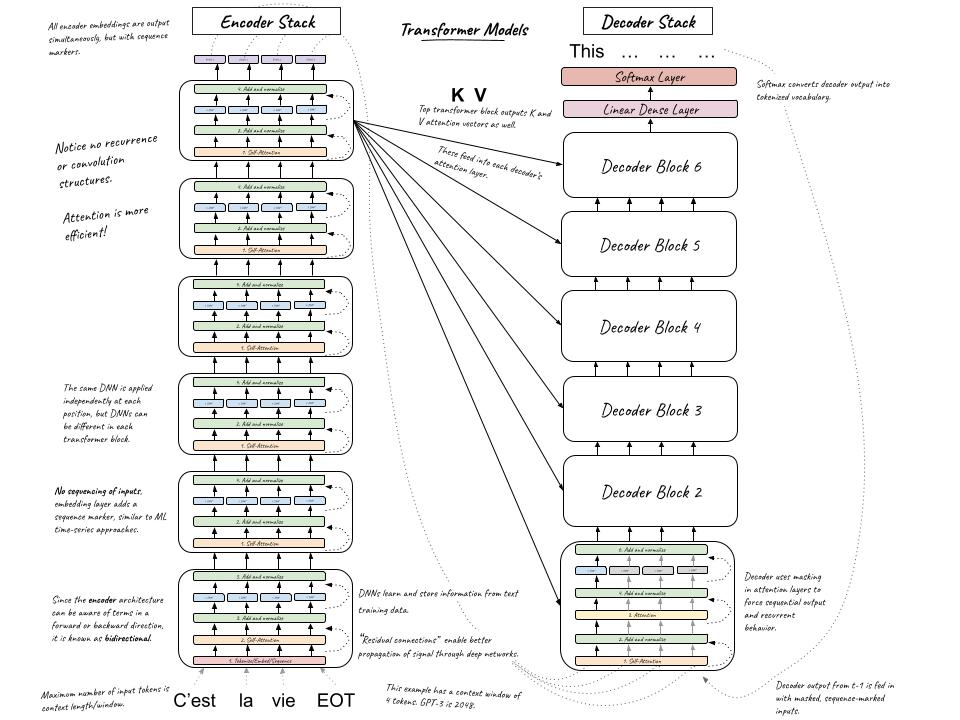
\includegraphics[width=.87\linewidth]{asset/transformer_basics.jpg}
\visualdescription{An encoder--decoder transformer stacks attention and feed-forward blocks.}
\end{columns}
\slidesource{\textcite{Vaswani2017AttentionAllYou}, \href{https://arxiv.org/abs/1706.03762}{transformer architecture}}
\end{frame}

\begin{frame}{Generation}
\small
\begin{columns}[c]
\column{.50\textwidth}
At step $t$, the model produces logits $\mathbf s_t$ and a categorical distribution:
\[
p(x_{t+1}\mid x_{\le t})=\operatorname{softmax}(\mathbf s_t/T).
\]
\begin{itemize}
  \item Greedy decoding chooses the highest-probability token.
  \item Lower $T$ sharpens the probability distribution; higher $T$ flattens it. Top-$k$ and top-$p$ truncate the candidate set.
  \item The chosen ID is appended and the forward pass repeats until a stop condition.
\end{itemize}
\vspace{.35em}
{\tiny\color{hrgray}Visual: A GPT-2-style decoder maps contextual token representations to next-token probabilities.\par}
\vspace{.35em}
{\tiny\color{hrgray}Source: \textcite{Holtzman2020CuriousCase}, \href{https://openreview.net/forum?id=rygGQyrFvH}{decoding and nucleus sampling}.\par}
\column{.46\textwidth}
\centering
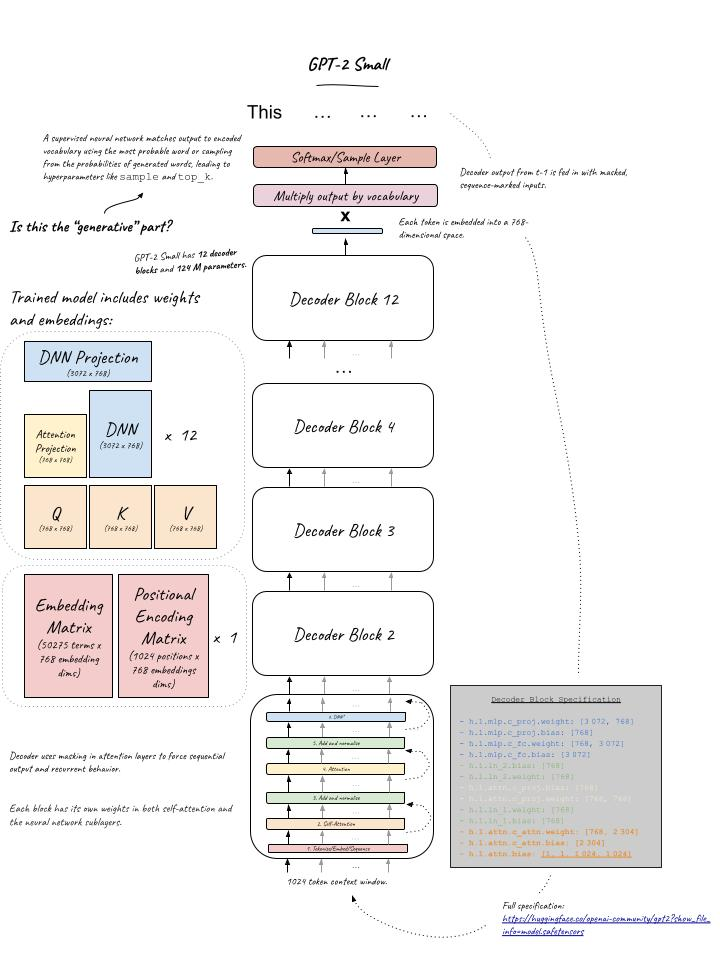
\includegraphics[height=.93\textheight]{asset/gpt2_generation.jpg}
\end{columns}
\vspace*{-.9em}
\end{frame}

\begin{frame}{Inference-time scaling trades resources for solution quality}
\small
\begin{columns}[T]
\column{.45\textwidth}
Instead of changing model weights, an inference procedure can spend more compute by:
\begin{itemize}
  \item generating longer deliberations;
  \item sampling several candidate solutions;
  \item verifying, ranking, or revising candidates;
  \item searching a tree of possible continuations.
\end{itemize}
Returns can plateau or reverse: the best allocation depends on task difficulty and the verifier.
\column{.51\textwidth}
\centering
{\scriptsize\textbf{Multiple candidates and selection}\par}
\vspace{.15em}
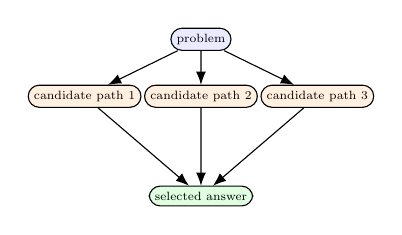
\begin{tikzpicture}[>=Latex,scale=.62,transform shape,every node/.style={font=\scriptsize}]
\node[draw,rounded corners,fill=blue!8] (p) {problem};
\node[draw,rounded corners,fill=orange!12,below left=7mm and 6mm of p] (r1) {candidate path 1};
\node[draw,rounded corners,fill=orange!12,below=7mm of p] (r2) {candidate path 2};
\node[draw,rounded corners,fill=orange!12,below right=7mm and 6mm of p] (r3) {candidate path 3};
\node[draw,rounded corners,fill=green!12,below=16mm of r2] (a) {selected answer};
\draw[->] (p)--(r1); \draw[->] (p)--(r2); \draw[->] (p)--(r3);
\draw[->] (r1)--(a); \draw[->] (r2)--(a); \draw[->] (r3)--(a);
\end{tikzpicture}

\vspace{.35em}
{\scriptsize\textbf{Compute--quality tradeoff}\par}
\vspace{.1em}
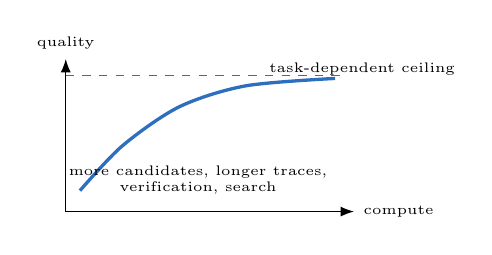
\begin{tikzpicture}[x=.60cm,y=.38cm,>=Latex,every node/.style={font=\tiny}]
  \draw[->] (0,0)--(6.1,0) node[right]{compute};
  \draw[->] (0,0)--(0,5.1) node[above]{quality};
  \draw[very thick,brand] plot[smooth] coordinates {(0.3,.7) (1.2,2.2) (2.4,3.5) (3.8,4.2) (5.7,4.45)};
  \draw[dashed,hrgray] (0,4.55)--(5.8,4.55);
  \node[align=center] at (2.8,1.05) {more candidates, longer traces,\\verification, search};
  \node[anchor=west] at (4.1,4.75) {task-dependent ceiling};
\end{tikzpicture}
\visualdescription{Top: several candidate reasoning paths feed a selected answer. Bottom: additional inference compute can improve solution quality, with diminishing returns.}
\end{columns}
\slidesource{\textcite{Snell2024ScalingLLMTestTime}, \href{https://arxiv.org/abs/2408.03314}{test-time compute}; \textcite{PromontoryAI2026Practicum}, \href{https://promontoryai.com/gwu-practicum-26/}{reasoning effort and cost}}
\end{frame}

\begin{frame}{Reasoning methods allocate intermediate computation}
\small
\begin{columns}[T]
\column{.46\textwidth}
\begin{itemize}
  \item Chain-of-thought prompting uses intermediate text to improve performance on some multi-step tasks.
  \item Reasoning models use training and decoding procedures that spend additional computation before returning a final answer.
\end{itemize}
\vspace{1.3em}
\begin{block}{A trace is not a causal explanation}
\footnotesize A plausible intermediate trace can still support a wrong answer and may not faithfully reveal the model's internal cause.
\end{block}
\column{.50\textwidth}
\centering
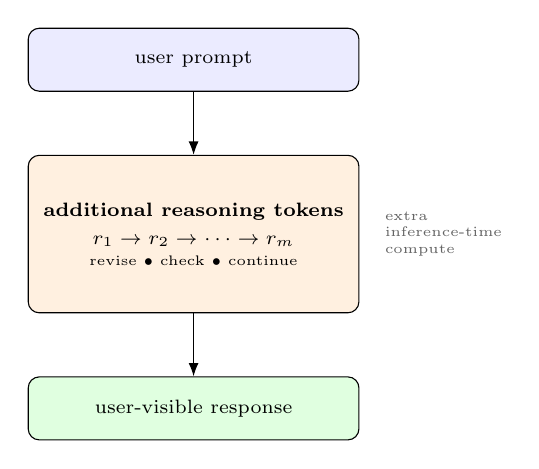
\begin{tikzpicture}[>=Latex,node distance=8mm,every node/.style={font=\scriptsize},box/.style={draw,rounded corners,align=center,minimum width=42mm,minimum height=8mm}]
\node[box,fill=blue!8] (p) {user prompt};
\node[box,fill=orange!12,below=of p,minimum height=20mm] (r) {\textbf{additional reasoning tokens}\\[.25em]
$r_1\rightarrow r_2\rightarrow\cdots\rightarrow r_m$\\[-.05em]
{\tiny revise $\bullet$ check $\bullet$ continue}};
\node[box,fill=green!12,below=of r] (a) {user-visible response};
\draw[->] (p)--(r);
\draw[->] (r)--(a);
\node[font=\tiny,text=hrgray,align=left,right=2mm of r] {extra\\inference-time\\compute};
\end{tikzpicture}
\visualdescription{A reasoning model generates additional reasoning tokens before issuing a user-visible response.}
\end{columns}
\slidesource{\textcite{Wei2022ChainThoughtPrompting}, \href{https://arxiv.org/abs/2201.11903}{chain-of-thought prompting}; \textcite{PromontoryAI2026Practicum}, \href{https://promontoryai.com/gwu-practicum-26/}{GWU practicum guest lecture}}
\end{frame}

\begin{frame}{Alignment shapes behavior after pretraining}
\footnotesize
\begin{columns}[c]
\column{.40\textwidth}
\begin{itemize}
  \item \textbf{Pretraining:} learn next-token prediction.
  \item \textbf{Supervised fine-tuning:} imitate curated demonstrations.
  \item \textbf{Preference alignment:} learn from comparisons or rewards through RLHF, DPO, or related objectives.
  \item \textbf{Evaluation and safeguards:} test intended behavior, misuse, and regressions.
\end{itemize}
Alignment changes behavior; it does not guarantee truth, safety, or universal agreement.
\column{.56\textwidth}
\centering
\vspace*{2em}
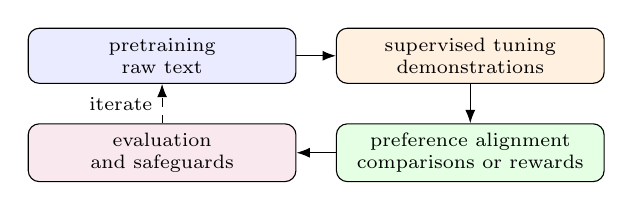
\begin{tikzpicture}[>=Latex,node distance=5mm,every node/.style={font=\scriptsize},box/.style={draw,rounded corners,minimum width=34mm,minimum height=7mm,align=center}]
\node[box,fill=blue!8] (pre) {pretraining\\raw text};
\node[box,fill=orange!12,right=of pre] (sft) {supervised tuning\\demonstrations};
\node[box,fill=green!10,below=of sft] (pref) {preference alignment\\comparisons or rewards};
\node[box,fill=purple!9,left=of pref] (eval) {evaluation\\and safeguards};
\draw[->] (pre)--(sft); \draw[->] (sft)--(pref); \draw[->] (pref)--(eval);
\draw[->,dashed] (eval)--node[left]{iterate}(pre);
\end{tikzpicture}
\visualdescription{Alignment iterates through pretraining, supervised tuning, preference optimization, and evaluation.}
\vspace*{-2em}
\end{columns}
\slidesource{\textcite{Ouyang2022TrainingLanguageModels}, \href{https://arxiv.org/abs/2203.02155}{RLHF}; \textcite{Rafailov2023DirectPreferenceOptimization}, \href{https://arxiv.org/abs/2305.18290}{DPO}; \textcite{PromontoryAI2026Practicum}, \href{https://promontoryai.com/gwu-practicum-26/}{GWU practicum guest lecture}}
\end{frame}

\begin{frame}{Putting the pieces together}
\scriptsize
\begin{columns}[T]
\column{.51\textwidth}
\begin{itemize}
  \setlength{\itemsep}{.15em}
  \item \textbf{Tokenization and encoding} turn text into token IDs---numbers a model can process.
  \item \textbf{Embeddings} map token IDs to learned vectors that represent useful features and similarities. Positional information represents token order.
  \item {\linespread{.92}\selectfont \textbf{Transformer blocks} combine self-attention, position-wise neural networks, residual connections, and normalization to update those vectors.\par}
  \begin{itemize}
    \scriptsize
    \setlength{\itemsep}{0em}
    \item Feed-forward networks process each token position separately.
    \item Self-attention mixes information across permitted positions; a causal language model uses the current and earlier tokens.
    \item Stacked blocks learn increasingly complex contextual patterns. Many LLMs use decoder-only stacks.
  \end{itemize}
\end{itemize}
\column{.45\textwidth}
\begin{itemize}
  \setlength{\itemsep}{.2em}
  \item \textbf{Prediction} maps the final hidden vector to one score per vocabulary token, then converts the scores into probabilities.
  \item \textbf{Generation} selects or samples a next token, appends it to the sequence, and repeats the process.
  \item \textbf{Inference-time scaling and reasoning} can spend more computation on longer reasoning, multiple candidates, search, or verification before returning a response.
  \item \textbf{Alignment} steers next-token behavior toward human instructions, preferences, and safety goals, but does not guarantee truth or safety.
\end{itemize}
\end{columns}
\end{frame}

\section{References}

\begin{frame}[t]{References}
\scriptsize
\printbibliography[heading=none,category=referencesone]
\end{frame}

\begin{frame}[t]{References}
\scriptsize
\printbibliography[heading=none,category=referencestwo]
\end{frame}
\end{document}
